\chapter{Antecedentes}
\begin{center}
Este capitulo está dedicado a presentar los resultados principales de \citep{alma991031505829703276} \& \citep{Barot1999ACO} que permiten caracterizar a las formas $\DynA_{n}$
\end{center}

\section{EL MÉTODO DE LAS INFLACIONES}\label{sec:2.1}

\paragraph{}
La demostración del teorema \ref{teorema:1.6} aparece en \citep{alma991031505829703276} y hace uso implícito de un algoritmo que describiremos aqui.

\paragraph{}
La idea intuitiva es pasar mediante cambios de variable enteros de la forma unitaria conexa $q$ a la forma unitaria $q'$, donde $\textbf{B}_{q'}$ no contiene aristas punteadas. Si $q$ es definida positiva entonces por lemma \ref{lema:1.3} $q'$ tambien es definidad positiva; luego como $q'$ solamente contiene aristas solidas entonces por lema \ref{lema:1.7} se sigue que cada una de sus componentes conexas debe ser una gráfica de Dynkin(figura \ref{figura:1.2}). El procedimiento para encontrar dicha forma cuadrática $q'$ es el \textit{método de las inflaciones} y es el tema de esta sección.\\

\textbf{INFLACIONES Y DEFLACIONES}

\paragraph{}
Tomemos matrices elementales $E_{sr}^{d}$, cuya transformación lineal 
\begin{equation*}
    T_{sr}^{d}\left(A\right) = E_{sr}^{d}A
\end{equation*}

equivale a sumar $d$ veces el renglón $s$ de $A$ al renglón $r$ de $A$. Dado que la matriz inversa de $E_{sr}^{d}$ es $E_{sr}^{-d}$, notamos que $E_{sr}^{d}$ es $\mathrm{Z}$-invertible si y solamente si $d$ es un número entero.

\paragraph{}
Consideremos el cambio de variable entero $\overrightarrow{y} = E_{sr}^{d}\overrightarrow{x}$, entonces

\begin{equation*}
    \begin{bmatrix}
    y_{1}\\
    \vdots\\
    y_{r}\\
    \vdots\\
    y_{n}&
    \end{bmatrix} = E_{sr}^{d}\begin{bmatrix}
    x_{1}\\
    \vdots\\
    x_{r}\\
    \vdots\\
    x_{n}
    \end{bmatrix} = \begin{bmatrix}
     x_{1}\\
    \vdots\\
    x_{r} + dx_{s}\\
    \vdots\\
    x_{n}
    \end{bmatrix}
\end{equation*}

y por tanto podemos concluir que $T_{sr}^{d}$ como cambio de variable tiene el mismo efecto que sustituir $x_{r} \leftarrow x_{r} + dx_{s}$.\\ ¿Qué efecto tiene $T_{sr}^{d}$ si sobre una forma unitaria $q$?. Supongamos que $q$ tiene matriz asociada $A = \left[a_{ij}\right]$ y sea

\begin{equation*}
    q'(\overrightarrow{x}) = \frac{1}{2}\left(E_{rs}^{d}\right)^{T} A E_{sr}^{d}
\end{equation*}

Dado que $E_{sr}^{d}$ es la matriz identidad salvo por la d en la posición $(s, r)$-ésima, entonces $\left(E_{sr}^{d}\right)^{T} = E_{sr}^{d}$. Por lo tanto $\left(E_{sr}^{d}\right)^{T}$ tiene el efecto de sumar $d$ veces el renglón $r$ al renglón $s$. Por otra parte $E_{sr}^{d}$ multiplicado por la derecha tiene el efecto de sumar $d$ veces la columna $r$ a la columna $s$, por lo tanto la matriz $C = \left(E_{sr}^{d}\right)^{T} A E_{sr}^{d}$ está dada por

\begin{equation}
c_{ij} = \left \{ 
    \begin{matrix} 
    a_{ij} & \mbox{si } i \neq s \mbox{ y } j \neq s\\
    a_{sj} + da_{rj} & \mbox{si } i = s \mbox{ pero } j \neq s\\ 
    a_{is} + da_{ir} & \mbox{si } j = s \mbox{ pero } i \neq s\\
    d^{2}a_{rr} + d(a_{sr} + a_{rs}) + a_{ss} & \mbox{si } i = s \mbox{ y } j = s
    \end{matrix}\right.
    \label{ecuacion:2.1}
\end{equation}

$E_{rs}^{d}$ define un cambio de variable entero, por lo que $C$ es la matriz asociada a alguna forma cuadrática entera, aunque no necesariamente unitaria. Para que $q'(\overrightarrow{x}) = \frac{1}{2}\overrightarrow{x}^{T}C\overrightarrow{x}$ sea una forma unitaria es necesario que $c_{ss} = 2$, o lo que es lo mismo (con $a_{rr} = a_{ss} = 2$ y $a_{rs} = a_{sr}$:

\begin{equation*}
    2d^{2} + 2da_{rs} + 2 = 2.
\end{equation*}

\paragraph{}
Esta ecuación tiene dos soluciones: $d = 0$y $d = -a_{rs}$. Estas soluciones se resumen en el siguiente lema:

\begin{lemma}
Si $q$ es una forma unitaria entonces $q \circ T_{rs}^{d}$ es una forma unitaria si y solo si $q_{rs} = q_{sr} = -d$.
\label{lema:2.1}
\end{lemma}

\begin{corollary}
Si $q$ es una forma unitaria simple entonces $q \circ T_{rs}^{d}$ es una forma unitaria para un $d \neq 0$ en cualquiera de estos dos casos y solamentes estos dos:
\label{corolario:2.2}
\end{corollary}

\begin{enumerate}
    \item $d = 1$ y $\textbf{B}_{q}$ contiene una arista punteada entre los vértices $x_{r}$ y $x_{s}$.
    \item $d = -1$ y $\textbf{B}_{q}$ contiene a una arista sólida entre los vertices $x_{r}$ y $x_{s}$.
\end{enumerate}

\paragraph{}
Este corolario no garantiza que $q \circ T_{rs}^{d}$ sea simple; en este caso por corolario 1.9 vemos que esto ocurre solamente cuando $q$ (que es $\mathrm{Z}$-equivalente a $q \circ T_{rs}^{d}$) no es definida positiva.

\paragraph{}
Con base al corolario anterior se justifica que definamos la transformación de \textbf{inflación} como

\begin{equation*}
    T_{rs}^{-} = T_{rs}^{-1}
\end{equation*}

y la transformación de la \textbf{deflación} como

\begin{equation*}
    T_{rs}^{+} = T_{rs}^{1}
\end{equation*}

\paragraph{}
El corolario anterior dice que la inflación $T_{rs}^{-}$ se puede aplicar solamente cuando $\textbf{B}_{q}$ contiene a la arista punteada $x_{r} \tikz[baseline=-0.1ex]\draw [dotted] (0,0.05) -- (1,0.05); x_{s}$ mientras que $T_{rs}^{+}$ solamente cuando $\textbf{B}_{q}$ contiene a la arista sólida $x_{r}  \rule[1mm]{5mm}{0.1mm} x_{s}$. A partir de la ecuación (\ref{ecuacion:2.1}), y del hecho de que la matriz es simétrica. Podemos interpretar las inflaciones y deflaciones como un algoritmo de reconexión sobre la gráfica $\textbf{B}_{q}$ (bajo las condiciones del corolario anterior) que consiste de cuatro pasos:

\begin{enumerate}
    \item \textit{Duplicar}: Generar una copia de las aristas que inciden en $x_{i}$ excepto la arista que conecta $x_{i}$ con $x_{j}$.
    \item \textit{Invertir}: En caso de una inflación reeplazar $x_{i} \tikz[baseline=-0.1ex]\draw [dotted] (0,0.05) -- (1,0.05); x_{j}$ por $x_{i} \rule[1mm]{5mm}{0.1mm} x_{j}$ y para cada arista duplicada del paso anterior intercambiar las aristas punteadas con sólidas y viceversa. En caso de una deflación simplemente reemplazar $x_{i} \rule[1mm]{5mm}{0.1mm} x{j}$ por $x_{i} \tikz[baseline=-0.1ex]\draw [dotted] (0,0.05) -- (1,0.05); x_{j}$
    \item \textit{Arrastrar}: Cada una de las aristas duplicadas se desconecta de su $x_{i}$ y se reconecta en $x_{j}$.
    \item \textit{Simplificar}: Si existen dos aristas $x_{i} \tikz[baseline=-0.1ex]\draw [dotted] (0,0.05) -- (1,0.05); x_{j}$ y $x_{i} \rule[1mm]{5mm}{0.1mm} x{j}$ incidentes en $x_{r}$ y $x_{j}$,  se borran.
\end{enumerate}

\paragraph{}
Por ejemplo, consideremos la forma cuadrática $q$ de la ecuación (\ref{ecuacion:1.5}) y ordenemos a las variables como $(w,x,y,z)$. Entonces para aplicar $T_{23}^{-}$ podemos calcular $\left(E_{23}^{-1}\right)^{T}~A~E_{23}^{-1}$ donde $A$ es la matriz asociada a $q$.\\

\begin{equation*}
    \begin{bmatrix}
    1 &  0  & 0 & 0\\
    0 &  1  & 0 & 0\\
    0 & -1  & 1 & 0\\
    0 &  0  & 0 & 1\\
    \end{bmatrix} \begin{bmatrix}
     2 & -1 &   0 &   0\\
    -1 &  2 &   1 &  -1\\
     0 &  1 &   2 &  -1\\
     0 & -1 & -1 &    2\\
    \end{bmatrix} \begin{bmatrix}
    1 &  0  &    0 & 0\\
    0 &  1  &  -1  & 0\\
    0 &  0  &   1  & 0\\
    0 &  0  &   0  & 1\\
    \end{bmatrix} = 
    \begin{bmatrix}
     2 & -1 &  1 &    0\\
    -1 &  2 & -1 &  -1\\
     1 & -1 &  2 &    0\\
     0 & -1 &  0 &   2\\
    \end{bmatrix}
\end{equation*}

La matriz resultante nos describe la misma forma cuadrática que se hubiera obtenido reemplazando $y \rightarrow y - z $; en efecto:

\begin{equation*}
x^{2} + (y - z)^{2} + z^{2} + w^{2} - x(y - z) + (y - z)z  - (y - z)w - zw = x^{2} + y^{2} + z^{2} + w^{2} -xy +xz - yz -yw
\end{equation*}

Tambien se puede hacer el cambio de variable de manera gráfica como se ilustra a continuación en la figura (\ref{figura:2.1})

\begin{figure}[h]
    \begin{subfigure}[b]{0.3\textwidth}
       \begin{minipage}{7cm}
        \centering% El subgrafo está centrado
        \begin{tikzpicture}
	    \node (v1) at (1.9914399682732804, 0.9921104441137079) {$x$};
	    \node (v2) at (0.9905576274421105, 0.7146057713195639) {$y$};
	    \node (v3) at (0.0, 0.9512105498862511) {$z$};
	    \node (v4) at (0.26505088954607003, 0.0) {$w$};
	    \draw (v1) -- (v2);
	    \draw[dotted] (v2) -- (v3);
	    \draw (v2) -- (v4);
	    \draw (v3) -- (v4);
        \end{tikzpicture}
        \end{minipage}
        \caption{Original}
     \end{subfigure}
     \begin{subfigure}[b]{0.3\textwidth}
        \begin{minipage}{7cm}
        \centering% El subgrafo está centrado
        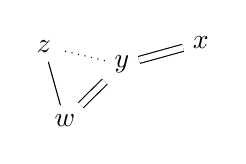
\begin{tikzpicture}
	\node (v1) at (1.9914399682732804, 0.9921104441137079) {$x$};
	\node (v2) at (0.9905576274421105, 0.7146057713195639) {$y$};
	\node (v3) at (0.0, 0.9512105498862511) {$z$};
	\node (v4) at (0.26505088954607003, 0.0) {$w$};
	 \draw[dotted] (v2) -- (v3);
	 \draw[double, double distance = 0.5ex] (v1) -- (v2);
	 \draw[double, double distance = 0.5ex] (v2) -- (v4);
	 \draw (v3) -- (v4);
        \end{tikzpicture}
        \end{minipage}
        \caption{Duplicar}
     \end{subfigure}
     \begin{subfigure}[b]{0.3\textwidth}
        \begin{minipage}{7cm}
        \centering% El subgrafo está centrado
        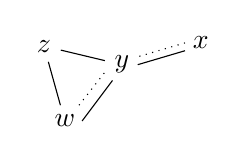
\begin{tikzpicture}
	\node (v1) at (1.9914399682732804, 0.9921104441137079) {$x$};
	\node (v2) at (0.9905576274421105, 0.7146057713195639) {$y$};
	\node (v3) at (0.0, 0.9512105498862511) {$z$};
	\node (v4) at (0.26505088954607003, 0.0) {$w$};
	 \draw[dotted] (1.7914399682732804, 0.9921104441137079) to (1.1905576274421105, 0.8146057713195639);
	\draw (1.7914399682732804, 0.8921104441137079) to (1.1905576274421105, 0.7146057713195639);
	 \draw[dotted] (0.44505088954607003, 0.2) to (0.7705576274421105, 0.6146057713195639);
	\draw (0.48505088954607003, 0.0) to (0.8705576274421105, 0.5146057713195639);
	 \draw (v2) -- (v3);
	 \draw (v3) -- (v4);
        \end{tikzpicture}
        \end{minipage}
        \caption{Invertir}
     \end{subfigure}
     \vfill
     \begin{subfigure}[b]{0.5\textwidth}
        \begin{minipage}{7cm}
        \centering% El subgrafo está centrado
        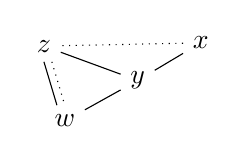
\begin{tikzpicture}
	\node (v1) at (1.9914399682732804, 0.9921104441137079) {$x$};
	\node (v2) at (1.1905576274421105, 0.5146057713195639) {$y$};
	\node (v3) at (0.0, 0.9512105498862511) {$z$};
	\node (v4) at (0.26505088954607003, 0.0) {$w$};
	 \draw (v1) -- (v2);
	 \draw[dotted] (v1) -- (v3);
	 \draw (v2) -- (v3);
	 \draw (v2) -- (v4);
	 \draw (0.0, 0.7512105498862511) to (0.16505088954607003, 0.2);
	 \draw[dotted] (0.1, 0.7512105498862511) to (0.26505088954607003, 0.2);
        \end{tikzpicture}
        \end{minipage}
        \caption{Arrastrar}
     \end{subfigure}
      \begin{subfigure}[b]{0.5\textwidth}
         \begin{minipage}{7cm}
        \centering% El subgrafo está centrado
        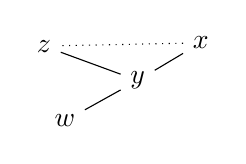
\begin{tikzpicture}
	\node (v1) at (1.9914399682732804, 0.9921104441137079) {$x$};
	\node (v2) at (1.1905576274421105, 0.5146057713195639) {$y$};
	\node (v3) at (0.0, 0.9512105498862511) {$z$};
	\node (v4) at (0.26505088954607003, 0.0) {$w$};
	 \draw (v1) -- (v2);
	 \draw (v2) -- (v3);
	 \draw[dotted] (v1) -- (v3);
	 \draw (v2) -- (v4);
        \end{tikzpicture}
        \end{minipage}
        \caption{Simplificar}
     \end{subfigure}
     \caption{Ejemplo de una inflación.}
    \label{figura:2.1}
\end{figure}

\textbf{DESCRIPCIÓN Y JUSTIFICACIÓN}

\paragraph{}
El método que aparece en \citep{alma991031505829703276} consiste en aplicar sucesivamente inflaciones como se indica en el algoritmo \ref{alg:algoritmoInflaciones} tanto como sea posible, es decir, hasta que no haya más aristas punteadas.

\begin{algorithm}[!ht]
\DontPrintSemicolon
  \While{exista una arista punteada $x_{r} \tikz[baseline=-0.1ex]\draw [dotted] (0,0.05) -- (1,0.05); x_{s}$ con $r \le s$ en $\textbf{B}_{q}$:}
   {
   		$q = q \circ T_{rs}^{-}$\;
   		\If{para algun coeficiente $q_{ij}$ se tiene $\left|q_{ij}\right| \ge 1:$}{
   			\Return no es positiva\;
   		}
   		
   		
   }
   \For{cada componente conexa $\mathcal{C}$ de $\textbf{B}_{q}$}{
   	$n =$ número de vértices que contiene $\mathcal{C}$\;
   	\If{$\mathcal{C}$ no es isomorfa a $\DynA_{n}, \DynD_{n}, \DynE_{6}, \DynE_{7}, \DynE_{8}$}
   		\Return no es positiva\;
   
   }
 \Return es positiva y es de tipo Dynkin $\textbf{B}_{q}$
\caption{Inflaciones(q)}\label{alg:algoritmoInflaciones}
\end{algorithm}

Veamos como funciona este algoritmo sobre la forma cuadrática de la ecuacion (\ref{ecuacion:1.5}).
\begin{enumerate}
\item Comenzamos con la forma unitaria
\begin{center}
\begin{tikzpicture}[scale=1.7]
	    \node (v1) at (1.9914399682732804, 0.9921104441137079) {$x$};
	    \node (v2) at (0.9905576274421105, 0.7146057713195639) {$y$};
	    \node (v3) at (0.0, 0.9512105498862511) {$z$};
	    \node (v4) at (0.26505088954607003, 0.0) {$w$};
	    \draw (v1) -- (v2);
	    \draw[dotted] (v2) -- (v3);
	    \draw (v2) -- (v4);
	    \draw (v3) -- (v4);
\end{tikzpicture}
\end{center}
$x^{2} + y^{2} + z^{2} + w^{2} - xy + yz - yw - zw$
\item Tenemos a la arista  $y \tikz[baseline=-0.1ex]\draw [dotted] (0,0.05) -- (1,0.05); z$ y aplicamos $T_{23}^{-}$ para obtener
\begin{center}
\begin{tikzpicture}[scale=1.7]
	    \node (v1) at (1.9914399682732804, 0.9921104441137079) {$x$};
	    \node (v2) at (0.9905576274421105, 0.7146057713195639) {$y$};
	    \node (v3) at (0.0, 0.9512105498862511) {$z$};
	    \node (v4) at (0.26505088954607003, 0.0) {$w$};
	    \draw (v1) -- (v2);
	    \draw[dotted] (v1) -- (v3);
	    \draw (v2) -- (v4);
	    \draw (v3) -- (v2);
\end{tikzpicture}
\end{center}
$x^{2} + y^{2} + z^{2} + w^{2} - xy + xz - yz - wy$
\item Tenemos a la arista  $x \tikz[baseline=-0.1ex]\draw [dotted] (0,0.05) -- (1,0.05); z$ y aplicamos $T_{13}^{-}$ para obtener
\begin{center}
\begin{tikzpicture}[scale=1.7]
	    \node (v1) at (1.9914399682732804, 0.9921104441137079) {$x$};
	    \node (v2) at (0.9905576274421105, 0.7146057713195639) {$y$};
	    \node (v3) at (0.0, 0.9512105498862511) {$z$};
	    \node (v4) at (0.26505088954607003, 0.0) {$w$};
	    \draw (v1) -- (v2);
	    \draw (v1) -- (v3);
	    \draw (v2) -- (v4);
\end{tikzpicture}
\end{center}
$x^{2} + y^{2} + z^{2} + w^{2} - xy - xz - wy$
\item Esta gráfica es isomorfa a $\DynA_{4}$, por lo tanto es el tipo Dynkin de la forma cuadrática (\ref{ecuacion:1.5}).
\end{enumerate}

\paragraph{}
Para terminar la demostración del teorema \ref{teorema:1.6} es necesario mostrar que si $q$ es una forma unitaria definida positiva entonces este algoritmo termina. Esto lo podemos resumir de la siguiente manera.\\
\begin{itemize}
    \item Decimos que $\overrightarrow{x} \in \mathrm{Z}^{n}$ es una \textbf{raíz} de la forma unitaria $q$ si $q(\overrightarrow{x}) = 1$.
    \item Primero mostramos que toda forma cuadrática se puede poner en la forma
    \begin{eqnarray*}
 q({\overrightarrow{x}}) &  =  & \lambda_{1}y_{1}^{2} + \lambda_{2}y_{2}^{2} + \cdots + \lambda_{n}y_{n}^{2} \\
 y_{i} &  =  & x_{i}+ \sum_{j=i+1}^{n}\rho_{ij}x_{j}
    \end{eqnarray*}
    \item Vamos a suponer que $q$ es una forma unitaria positiva, y usando la expresión anterior mostraremos que $q$ tiene una cantidad finita de raíces. Más especificamente mostraremos que cada $x_{i}$ está acotada en el intervalo $\left[-\sigma, \sigma\right]$ para alguna constante $\sigma_{i}$.
    \item Encontraremos cierto subconjunto de raíces que crece con cada iteración del algoritmo \ref{alg:algoritmoInflaciones}. Como el conjunto de raíces es finito, la cantidad de iteraciones tambien.
\end{itemize}

La \textbf{reducción de Lagrange} es un método que nos permite llevar toda forma cuadrática a la forma (\ref{ecuacion:1.4}). Primero necesitamos recordar la fórmula de \textbf{completar cuadrados}:

\begin{equation}
\begin{split}
ax^{2} + bx + x & = a\left[x^{2} + \frac{b}{a}x \right] + c\\
 & = a\left[x^{2} + \frac{b}{a}x + \left(\frac{b}{2a}\right)^{2} - \left(\frac{b}{2a}\right)^{2} \right] + c\\
 & = a\left(x + \frac{b}{2a}\right)^{2} + \left(c - \frac{b^{2}}{4a} \right)
\end{split}
\label{ecuacion:2.2}
\end{equation}

\paragraph{}
Sea $q$ una forma unitaria sobre las variables $x_{k}, x_{k+1}, \ldots, x_{n}$. Para escribir $q\left(x_{k},\ldots,x_{k}\right)$ en la forma (\ref{ecuacion:1.4}) se hace los siguiente:

\begin{enumerate}
\item Si $q = q_{nn}x_{n}^{2}$ es una forma cuadratica en una variable entonces se definen $\lambda_{n} = q_{nn} = x_{n}$ y terminamos (en caso contrario seguimos).
\item Sea $\ell = k + 1$. Tomamos todos los terminos que contienen la variable $x_{k}$:
\begin{equation*}
q = q_{kk}x_{k}^{2} + \sum_{j=\ell}^{n}q_{kj}x_{k}x_{j} + r
\end{equation*}
donde $r = \sum_{i=\ell}^{n}q_{ii}x_{i}^{2} + \sum_{j=\ell+1}^{n}\sum_{i=\ell}^{j_1} q_{ij}x_{i}x_{j}$
\item Factorizamos $q_{k\ell}x_{k}$
 \begin{equation*}
q = q_{kk}x_{k}^{2} + q_{k\ell}x_{k}\left(\sum_{j=\ell}^{n}\frac{q_{kj}}{q_{k\ell}}x_{j}\right) + r
\end{equation*}
\item Complentando el cuadrado sustituyendo en la ecuación (\ref{ecuacion:2.2}) los valores de $a = q_{kk}, b= q_{k\ell}\left(\sum_{j=\ell}^{n}\frac{q_{kj}}{q_{k\ell}}x_{j}\right)$ y $c=0$
\begin{equation*}
q = q_{kk}\left(x + \sum_{j=\ell}^{n}\frac{q_{kj}}{2q_{kk}}x_{j}\right)^{2} - \frac{q_{k\ell}^{2}}{4q_{kk}}\left(\sum_{j=\ell}^{n}\frac{q_{kj}}{q_{k\ell}}x_{j}\right)^{2} + r
\end{equation*}
\item Se definen
\begin{equation*}
\lambda_{k} = q_{kk}
\end{equation*}
\begin{equation*}
y_{k} = x_{k} + \sum_{j=\ell}^{n}\frac{q_{kj}}{2q_{kk}}x_{j}
\end{equation*}
\begin{equation*}
q' = -\frac{q_{k\ell}^{2}}{4q_{kk}}\left(\sum_{j=\ell}^{n}\frac{q_{kj}}{q_{k\ell}}x_{j}\right)^{2} + r
\end{equation*}
Desarrollando el cuadrado en $q'$ vemos que $q'$ es una forma cuadrática sobre las variables $\left(x_{\ell},x_{\ell+1},\ldots,x_{n}\right)$ (una variable menos que $q$) y además 
\begin{equation*}
q = \lambda_{1}y_{1}^{2} + q'
\end{equation*}
\item Repetimos el mismo procedimiento para $q'$
\end{enumerate}

Este método es una demostración constructiva(e inductiva) de el siguiente lema:

\begin{lemma}
Toda forma cuadrática $q\left(\overrightarrow{x}\right)$ se puede reescribir como
\begin{equation}
\begin{split}
q\left(\overrightarrow{x}\right) & =\lambda_{1}y_{1}^{2} + \lambda_{2}y_{2}^{2} + \cdots + \lambda_{n}y_{n}^{2}\\
y_{i} & = x_{i} + \sum_{j=i+1}^{n}\rho_{ij}x_{j}
\end{split}
\label{ecuacion:2.3}
\end{equation}
\label{lema:2.3}
\end{lemma}

\begin{example}

 Sea $q\left(x_{1}, x_{2}, x_{3}\right) = x_{1}^{2} + 2x_{2}^{2} - 7x_{3}^{2} - 4x_{1}x_{2} + 8x_{1}x_{3}$ la primera iteración hace lo siguiente:
 
 \begin{equation*}
\begin{split}
q\left(x_{1}, x_{2}, x_{3}\right) & = x_{1}^{2} - 4x_{1}x_{2} + 8x_{1}x_{3} +  \underbrace{2x_{2}^{2} - 7x_{3}^{2}}_{r}\\
 & = \underbrace{1}_{a}x_{1}^{2} + x_{1} \underbrace{\left(-4\right)\left(x_{2} - 2x_{3}\right)}_{b} + \underbrace{2x_{2}^{2} - 7x_{2}^{2}}_{r}\\
 & = \underbrace{1}_{\lambda_{1}} \underbrace{\left(x_{1} - 2x_{2} + 4x_{3}\right)^{2}}_{y_{1}} \underbrace{- 4\left(x_{2} - 2x_{3}\right)^{2} + 2x_{2}^{2} - 7x_{3}^{2}}_{q'}\\
 & = \lambda_{1}y_{1}^{2} \underbrace{- 2x_{2}^{2} - 23x_{3}^{2} + 16x_{2}x_{3}}_{q'}
\end{split}
\end{equation*}

La segunda iteracíon funciona sobre $q'\left(x_{2}, x_{3} \right) = -2x_{2}^{2} - 23x_{3}^{2} + 16x_{2}x_{3}$:

\begin{equation*}
\begin{split}
q'\left(x_{2}, x_{3}\right) & = \underbrace{-2}_{a}x_{2}^{2} + x_{2}\underbrace{\left(16x_{3}\right)}_{b} - \underbrace{23x_{3}^{2}}_{r'}\\
 & = \underbrace{-2}_{\lambda_{2}}\underbrace{\left(x_{2} + 4x_{3}\right)^{2}}_{y_{2}} + \underbrace{9x_{3}^{2}}_{q''}\\
 & = \lambda_{2}y_{2} + \underbrace{9x_{3}^{2}}_{q''}
\end{split}
\end{equation*}

Finalmente en la tercera iteracíon opera sobre $q''\left(x_{3}\right) = 9x_{3}^{2}$, que es una forma cuadrática en una sola variable, por tanto $\lambda_{3} = 9$ y $y_{3} = x_{3}$. Así hemos reescrito a $q$ como 
\begin{equation*}
\begin{split}
q\left(x_{1}, x_{2}, x_{3}\right) & = y_{1}^{2} - 2y_{2}^{2} + 9y_{3}^{2}
\end{split}
\end{equation*}

donde 

\begin{equation*}
\begin{matrix}
y_{1} & =   x_{1}	& - 2x_{2}	&    4x_{3}\\
y_{2} & =		&     x_{2}	&  - 4x_{3}\\
y_{3} & =		&              	&      x_{3}
\end{matrix} 
\end{equation*}

\end{example}

\paragraph{}
Supongamos que $q$ es una forma unitaria definida positiva y que $\overrightarrow{x}$ es una raíz de $q$. Usando la reducción de Lagrange escribimos
\begin{equation*}
\begin{split}
q\left(\overrightarrow{x}\right) & =\lambda_{1}y_{1}^{2} + \lambda_{2}y_{2}^{2} + \cdots + \lambda_{n}y_{n}^{2}\\
y_{i} & = x_{i} + \sum_{j=i+1}^{n}\rho_{ij}x_{j}
\end{split}
\end{equation*}

Como $q$ es definida positiva entonces cada $\lambda_{i} > 0$. Más aún, como $\lambda_{1}y_{1}^{2} + \lambda_{2}y_{2}^{2} + \cdots + \lambda_{n}y_{n}^{2} = 1$ (porque habíamos supuesto que $\overrightarrow{x}$ es una raíz) entonces $\lambda_{i}y_{i}^{2} \leq 1$ para cada $i$.

\paragraph{}
Como $y_{n} = x_{n}$ entonces $\lambda_{n}x_{n}^{2} \leq 1$, de donde $|x_{n}| \leq \frac{1}{\sqrt{\lambda_{n}}}$. Definbiendo $\sigma_{n}=\frac{1}{\sqrt{\lambda_{n}}}$ se ha mostrado que $-\sigma_{n} \leq x_{n} \leq \sigma_{n}$ está acotada por alguna constante $\sigma_{k}$. En efecto, tenemos que 

\begin{equation*}
\lambda_{k}y_{k}^{2} = \lambda_{k}\left(x_{k} + \sum_{j=k+1}^{n}\rho_{kj}x_{j}\right)^{2} \leq 1
\end{equation*} 

de donde 

\begin{equation*}
\left|x_{k} + \sum_{j=k+1}^{n} \rho_{kj} x_{j}\right| \leq \frac{1}{\sqrt{}\lambda_{k}}
\end{equation*} 

Para continuar es necesaria la siguiente desigualdad:

\begin{equation}
\left|\sum_{i=1}^{m} a_{i}\right| \geq \left|a_{1}\right| - \sum_{i=2}^{m}\left|a_{i}\right|
\label{ecuacion:2.4}
\end{equation} 

para cualesquiera números reales $a_{1}, a_{2}, \ldots, a_{m}$. Esta desigualdad la demuestramos por inducción (el caso base $m=2$ establece que $\left|a_{1} + a_{2}\right| \geq \left|a_{1}\right| - \left|a_{2}\right|$ y se comprueba por casos; para el paso inductivo escribimos $\left|\sum_{i=1}^{m}a_{i}\right| \geq \left|\sum_{i=1}^{m-1}a_{i}\right| - \left|a_{m}\right|$ y aplicamos la inducción). Usando la desigualdad (\ref{ecuacion:2.4}) deducimos que 

\begin{equation*}
\left|x_{k}\right| - \sum_{j=k+1}^{n}\left| \rho_{kj}x_{j}\right| \leq \left|x_{k} + \sum_{j=k+1}^{n}\rho_{kj}x_{j}\right| \leq \frac{1}{\lambda_{k}}
\end{equation*} 

de donde despejando $\left|x_{k}\right|$ y usando que $x_{j} \leq \sigma_{j}$ con $\sigma_{j} \geq 0$, obtenemos

\begin{equation*}
\left|x_{k}\right| \leq \frac{1}{\sqrt{\lambda_{k}}} + \sum_{j=k+1}^{n}\left| \rho_{kj}x_{j}\right| \leq \frac{1}{\sqrt{\lambda_{k}}} + \sum_{j=k+1}^{n}\left|\rho_{kj}\right|\sigma_{j}
\end{equation*} 

Por lo tamto $\sigma_{k} = \frac{1}{\sqrt{\lambda_{k}}} + \sum_{j=k+1}^{n}\left|\rho_{kj}\right|\sigma_{j}$ es una constante tal que $-\sigma_{k} \leq x_{k} \leq \sigma_{k}$. Por inducción concluimos que si $\overrightarrow{x}$ es una raíz de $q$ entonces todo $x_{i}$ está acotado entre $-\sigma{i}$ y $\sigma_{i}$ para alguna constante $\sigma_{i}$. Como cada $x_{i}$ debe ser un número entero entre $-\sigma_{i}$ y $\sigma_{i}$ entonces concluimos el siguiente lema:

\begin{lemma}
Si $q$ es una forma unitaria positiva entonces su conjunto de raíces es finito.
\label{lema:2.4}
\end{lemma}

\paragraph{}
En lo siguiente denotaremos por $S(q)$ al conjunto finito de raíces de $q$, y por $R(q)$ al conjunto de raíces no negativas de $q$, en otras palabras:

\begin{equation*}
\begin{split}
S(q) & =\{ \overrightarrow{x} \in \mathbb{Z}^{n} | q\left(\overrightarrow{x}\right) = 1 \}\\
R(q) & = \{ \overrightarrow{x} \in \mathbb{N}^{n} | q\left(\overrightarrow{x}\right) = 1 \}
\end{split}
\end{equation*}

Claramente $R(q) \subseteq S(q)$.

\paragraph{}
Supongamos que $q$ es una forma unitaria positiva. Entonces $\textbf{B}_{q}$ es una gráfica simple y el algoritmo \ref{alg:algoritmoInflaciones} busca valores de $r$ y $s$ tales que existe una arista punteada $x_{r}$ \rule[1mm]{.1cm}{0.4pt} \rule[1mm]{.1cm}{0.4pt} \rule[1mm]{.1cm}{0.4pt} \rule[1mm]{.1cm}{0.4pt} $x_{s}$. Estos es lo mismo que decir que $q_{rs} = 1$ (ver Corolario \ref{corolario:1.9}). Sea $q' = q \circ T_{rs}^{-} $. Como la transformación $T_{rs}^{-}: \mathbb{Z}^{n} \rightarrow \mathbb{Z}^{n}$ está definida por una matriz $\mathbb{Z}$-invertible entonces $T_{rs}^{-}$ es invertible y su inversa es $T_{rs}^{+}$.

\paragraph{}
Supongamos que $\overrightarrow{x}$ es una raíz de $q$, entonces

\begin{equation*}
q'\left(T_{rs}^{+}\left(\overrightarrow{x}\right)\right) = q\left(T_{rs}^{-}\left(T_{rs}^{+} \left(\overrightarrow{x}\right)\right)\right) = q\left(\overrightarrow{x}\right) = 1
\end{equation*}

y por tanto $T_{rs}^{+}$ es una raíz de $q'$. Esto nos dice que de hecho $T_{rs}^{+}$ es una función biyectiva entre los conjuntos $S\left(q\right)$ y $S\left(q'\right)$, e inyectiva en los conjuntos $R\left(q\right)$ y $R\left(q'\right)$. De aqui concluimos que $\left|S\left(q\right)\right| =  \left|S\left(q'\right)\right|$ y que $\left|R\left(q\right)\right| \leq \left|R\left(q'\right)\right|$; mostraremos que esta desigualdad es estricta.

\paragraph{}
Denotamos con $\overrightarrow{e} = \left(d_{1}, d_{2},\dots,d_{n}\right)$ al vector tal que $d_{k}$ y $d_{i}$ para todo $i \neq k$. Sea $\overrightarrow{z} = \overrightarrow{e_{s}} - \overrightarrow{e_{r}} $. Notamos que 

\begin{equation*}
q\left(\overrightarrow{z}\right) = \left(-1\right)^{2} + 1^{2} + q_{rs}(-1)(1) = 1
\end{equation*}

por lo que $\overrightarrow{z} \in S\left(q\right)$ pero $\overrightarrow{z} \notin R\left(q\right)$ (porque tiene un $-1$ en la entrada $r$-ésima). Sin embargo $T_{rs}^{+}\left(\overrightarrow{z}\right) = \overrightarrow{e_{s}}$, es decir que $\overrightarrow{z} \in R\left(q'\right)$. Como $\overrightarrow{z} \in R\left(q'\right)$ pero $\overrightarrow{z} \notin R\left(q\right)$, entonces $\left|R\left(q\right)\right| < \left|R\left(q'\right)\right|$.\\

Finalmente, si denotamos por $q_{1}, q_{2},q_{3},\ldots$ a la sucesión de valores que toma la variable $q$ de el algoritmo \ref{alg:algoritmoInflaciones} entonces de lo anterior tenemos que\\

\begin{equation*}
\begin{split}
\left|S(q_{1})\right| & = \left|S(q_{2})\right| = \left|S(q_{3})\right| = \cdots\\
\left|R(q_{1})\right| & < \left|R\left(q_{2}\right)\right| < \left|R\left(q_{3}\right)\right| < \cdots 
\end{split}
\end{equation*}
Si estas sucesiones fuesen infinitas entonces eventualmente contradecimos que $R\left(q_{i}\right) \subseteq S\left(q_{i}\right)$, por lo tanto el algoritmo \ref{alg:algoritmoInflaciones} solamente puede hacer un número finito de iteraciones de ciclo \textbf{mientras}. Una breve vista al pseudocodigo nos muestra que esto ocurre cuando $\textbf{B}_{q}$ ya no contiene aristas punteadas, por lo tanto al término de este ciclo $\textbf{B}_{q}$ contiene solamente aristas sólidas. Como habiamos supuesto que $q$ es positiva y como cada $q_{i}$ es $\mathbb{Z}$-equivalente a $q$, entonces el lema \ref{lema:1.7} nos garantiza que cada componente conexa de $\textbf{B}_{q}$ es una gráfica de Dynkin.\\
Con esto concluye la demostración de el teorema \ref{teorema:1.6}.
\section{ENSAMBLAJE POR $\DynA$-BLOQUES}
\textbf{VISIÓN GENERAL DEL ENSAMBLE}
En \citep{Barot1999ACO} se aborda el problema de caracterizar las formas de tipo $\DynA_{n}$; pero en lugar de basarse en transformaciones, se basa en la construcción de las gráficas $\Delta$ tales que $q_{\Delta}$ es de tipo  $\DynA_{n}$. La idea es ir ``pegando'' ciertas gráficas como si fueran bloques de construcción. La estructura de estos bloques es muy sencilla: Se parte de dos conjuntos de vértices $V_{0}$ y $V_{1}$; entre los vértices $\left(u, v\right)$ hay una arista punteada $u\tikz[baseline=-0.1ex]\draw [dotted] (0,0.05) -- (1,0.05); v$ si ambos $u, v \in V_{0}$ o ambos $u, v \in V_{1}$, y una arista sólida $u \tikz[baseline=-0.1ex]\draw (0,0.05) -- (1,0.05); v$ en otro caso. A las gráficas así obtenidas les llamaremos $\DynA$-bloques y las denotaremos por $F_{m,m^{'}}$ donde $m = |V_{0}|$ y $m^{'} = |V_{1}|$ (pero acostumbramos a escribir $m \geq m^{'}$). La figura \ref{figura:2.3} muestra cómo dibujar un $\DynA$-bloque.\citep{AbarcaSoteloMarioAlberto2011Apds}\citep{Barot1999ACO}\\

\begin{figure}[h]
    \begin{subfigure}[b]{0.3\textwidth}
        \begin{minipage}{7cm}
        \centering% El subgrafo está centrado
        \begin{tikzpicture}
        \node (v0) at (1.56, 0.14) {1};
        \end{tikzpicture}
        \end{minipage}
        \caption{$F_{1,0}$}
     \end{subfigure}
     \begin{subfigure}[b]{0.3\textwidth}
        \begin{minipage}{7cm}
        \centering% El subgrafo está centrado
        \begin{tikzpicture}
        \node (v0) at (0.17, -0.93) {1};
        \node (v1) at (1.27, -0.93) {2};
        \node (v2) at (0.80, 0.23) {3};
        \draw[dotted] (v0) -- (v1);
        \draw[dotted] (v1) -- (v2);
        \draw[dotted] (v2) -- (v0);
        \end{tikzpicture}
        \end{minipage}
        \caption{$F_{3,0}$}
     \end{subfigure}
     \begin{subfigure}[b]{0.3\textwidth}
        \begin{minipage}{7cm}
        \centering% El subgrafo está centrado
        \begin{tikzpicture}
        \node (v0) at (2.47, -0.93) {1};
        \node (v1) at (1.27, -0.93) {2};
        \draw (v0) -- (v1);
        \end{tikzpicture}
        \end{minipage}
        \caption{$F_{1,1}$}
     \end{subfigure}
     \vfill
     \begin{subfigure}[b]{0.3\textwidth}
        \begin{minipage}{7cm}
        \centering% El subgrafo está centrado
        \begin{tikzpicture}
        \node (v0) at (1.07, -0.93) {1};
        \node (v1) at (-0.27, -0.93) {2};
        \draw[dotted] (v0) -- (v1);
        \end{tikzpicture}
        \end{minipage}
        \caption{$F_{2,0}$}
     \end{subfigure}
      \begin{subfigure}[b]{0.3\textwidth}
        \begin{minipage}{7cm}
        \centering% El subgrafo está centrado
        \begin{tikzpicture}
        \node (v0) at (0.37, 0.43) {1};
        \node (v1) at (1.07, -0.73) {2};
        \node (v2) at (-0.37, -0.73) {3};
        \draw (v0) -- (v1);
        \draw (v1) -- (v2);
        \draw[dotted] (v2) -- (v0);
        \end{tikzpicture}
        \end{minipage}
        \caption{$F_{2,1}$}
     \end{subfigure}
     \begin{subfigure}[b]{0.3\textwidth}
        \begin{minipage}{7cm}
        \centering% El subgrafo está centrado
        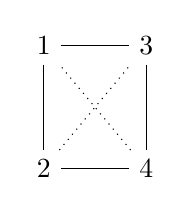
\begin{tikzpicture}
        \node (v0) at (1.27, 0.83) {1};
        \node (v1) at (1.27, -0.73) {2};
        \node (v2) at (2.57, 0.83) {3};
        \node (v3) at (2.57, -0.73) {4};
        \draw (v0) -- (v1);
        \draw[dotted] (v1) -- (v2);
        \draw (v2) -- (v3);
        \draw[dotted] (v3) -- (v0);
        \draw (v0) -- (v2);
        \draw (v3) -- (v1);
        \end{tikzpicture}
        \end{minipage}
        \caption{$F_{2,2}$}
     \end{subfigure}
     \begin{center}
      \begin{subfigure}[b]{0.8\textwidth}
        \centering% El subgrafo está centrado
        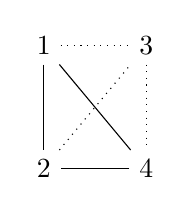
\begin{tikzpicture}
        \node (v0) at (1.27, 0.83) {1};
        \node (v1) at (1.27, -0.73) {2};
        \node (v2) at (2.57, 0.83) {3};
        \node (v3) at (2.57, -0.73) {4};
        \draw (v0) -- (v1);
        \draw[dotted] (v1) -- (v2);
        \draw[dotted] (v2) -- (v3);
        \draw (v3) -- (v0);
        \draw[dotted] (v0) -- (v2);
        \draw (v3) -- (v1);
        \end{tikzpicture}
        \caption{$F_{3,1}$}
     \end{subfigure}
     \end{center}
     \caption{Algunos ejemplos de $\DynA$-bloques.}
    \label{figura:2.2}
\end{figure}

\begin{figure}[H]
    \begin{subfigure}[b]{0.5\textwidth}
        \begin{minipage}{7cm}
        \centering% El subgrafo está centrado
         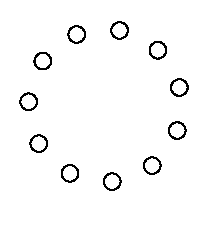
\includegraphics[height=.6\textwidth]{Figuras/A-bloque1}
        \end{minipage}
    \end{subfigure}
    \begin{subfigure}[b]{0.5\textwidth}
        \begin{minipage}{7cm}
        \centering% El subgrafo está centrado
         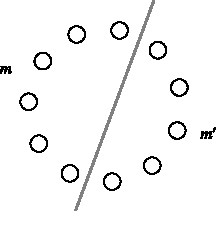
\includegraphics[height=.6\textwidth]{Figuras/A-bloque2}
        \end{minipage}
    \end{subfigure}
    \begin{subfigure}[b]{0.5\textwidth}
        \begin{minipage}{7cm}
        \centering% El subgrafo está centrado
         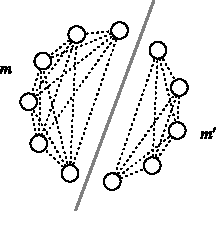
\includegraphics[height=.6\textwidth]{Figuras/A-bloque3}
        \end{minipage}
    \end{subfigure}
    \begin{subfigure}[b]{0.5\textwidth}
        \begin{minipage}{7cm}
        \centering% El subgrafo está centrado
         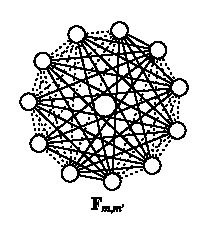
\includegraphics[height=.6\textwidth]{Figuras/A-bloque}
        \end{minipage}
    \end{subfigure}
    \caption{Como se construye un $\DynA$-bloque.}
    \label{figura:2.3}
\end{figure}

El resultado principal de \citep{Barot1999ACO} es que todas las formas unitarias de tipo $\DynA_{n}$ se construyen pegando $\DynA$-bloques sobre un árbol como se explica a continuación:

\begin{enumerate}
\item Se comienza con un árbol $T$ de vértices $\{1, 2, \ldots, t\}$ y a cada vértice $i \in T$ se le asocia un $\DynA$-bloque $\mathcal{B}_{i}$.
 \begin{figure}[H]
    \centering% El subgrafo está centrado
    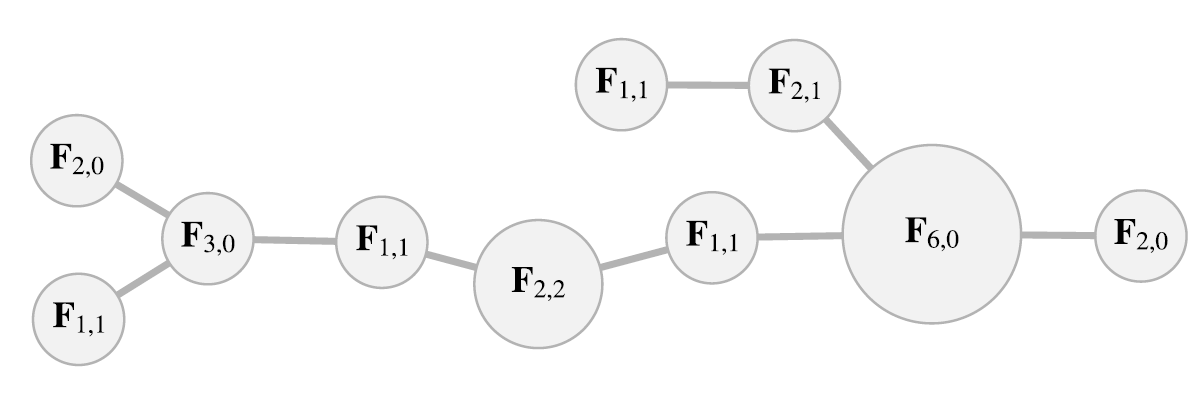
\includegraphics[height=.2\textwidth]{Figuras/graph.png}
\end{figure}
\item A cada arista $i \tikz[baseline=-0.1ex]\draw (0,0.05) -- (1,0.05); j \in T$ se le asocian los vértices $\sigma_{i}\left(i \tikz[baseline=-0.1ex]\draw (0,0.05) -- (1,0.05); j\right) \in \mathcal{B}_{i}$ y $\sigma_{j}\left(i \tikz[baseline=-0.1ex]\draw (0,0.05) -- (1,0.05); j \right)$ de manera que cada función $\sigma_{k}$ sea inyectiva.
 \begin{figure}[H]
    \centering% El subgrafo está centrado
    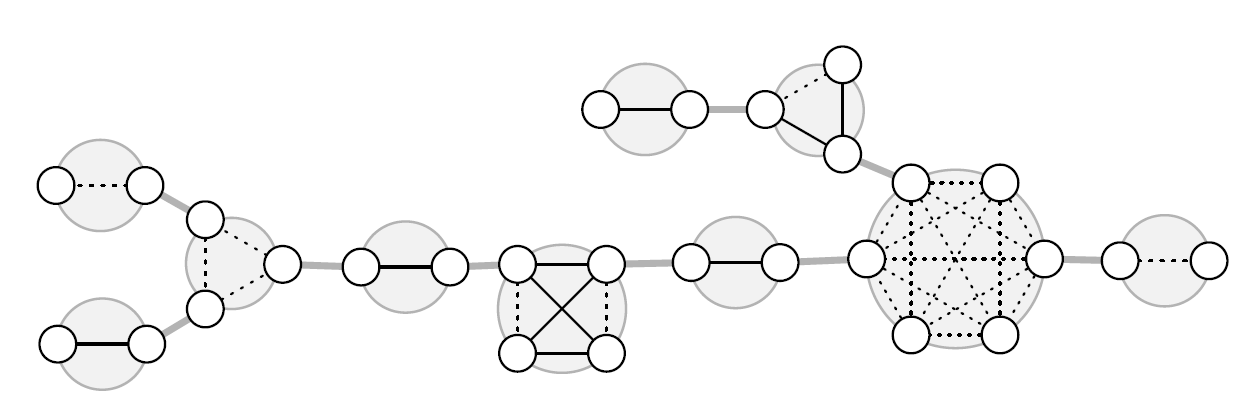
\includegraphics[height=.2\textwidth]{Figuras/graph1.png}
\end{figure}
\item Para cada arista $i \tikz[baseline=-0.1ex]\draw (0,0.05) -- (1,0.05); j \in T$ se identifican los vértices $\sigma_{i}\left(i \tikz[baseline=-0.1ex]\draw (0,0.05) -- (1,0.05); j\right)$ y $\sigma_{j}\left(i \tikz[baseline=-0.1ex]\draw (0,0.05) -- (1,0.05); j\right)$, es decir, se “pegan” para volverse uno solo. Continuando con este ejemplo obtenemos la figura 2.4
 \begin{figure}[H]
    \centering% El subgrafo está centrado
    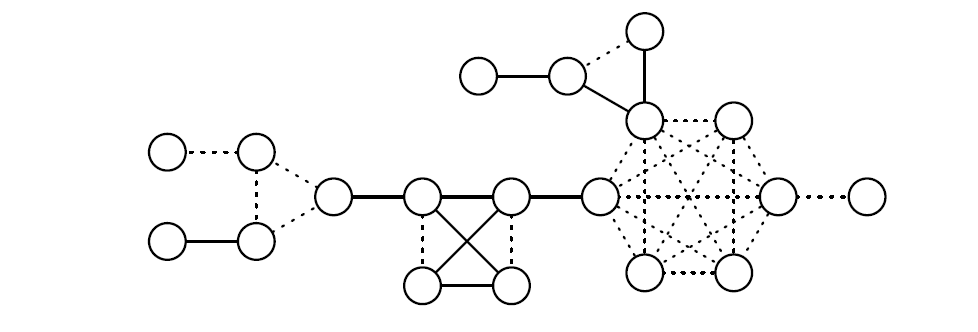
\includegraphics[height=.2\textwidth]{Figuras/graph3.png}
     \caption{Esta gráfica define a una forma de tipo $\DynA_{19}$}
    \label{figura:2.4}
\end{figure}
\end{enumerate}

\textbf{LOS $\DynA$-BLOQUES}

A continuación trataremos de justificar el ensamble de $\DynA$-bloques a partir del siguiente resultado tomado de \citep{article123}:
\begin{theorem}
Si $q_{G}$ es de tipo $\DynA_{n}$, y si $H$ es una subgráfica conexa inducida por $m$ vértices de $G$, entonces $q_{H}$ es de tipo $\DynA_{m}$.
\label{teorema:2.5}
\end{theorem}
Comencemos con un caso especial de gráficas: las gráficas circulares son aquellas en los que cada vértice está conectado con exactamente otros dos vértices. Nos interesa saber cuáles gráficas circulares definen formas cuadráticas de tipo $\DynA_{n}$. Ciertamente $F_{3,0}$ y $F_{2,1}$ son unas de estas (lo podemos comprobar usando el algoritmo \ref{alg:algoritmoInflaciones})\\

Trataremos de simplificar un poco el problema. Las gráficas circulares de la figura 2.5 definen formas $\mathbb{Z}$-equivalentes: podemos pasar de una a otra mediante las matrices elementales $E_{i}^{-1}$ de tamaño $n$. No es difícil comprobar que estas matrices tienen el efecto de intercambiar aristas sólidas con punteadas siempre que estas incidan en el vértice $x_{i}$. De hecho, este mismo razonamiento muestra que toda gráfica circular es equivalente a otra gráfica circular “estandarizada”, que consiste de aristas sólidas y posiblemente una sola arista punteada.\\

\begin{figure}[h]
    \begin{subfigure}[b]{0.3\textwidth}
      \begin{minipage}{7cm}
	\centering% El subgrafo está centrado
	    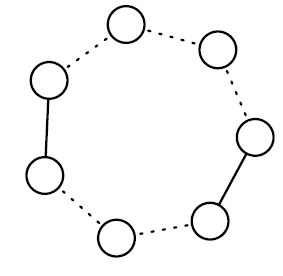
\includegraphics[height=.2\textwidth]{Figuras/graph4.png}
	 \end{minipage}
	\caption{}
     \end{subfigure}
     \begin{subfigure}[b]{0.3\textwidth}
        \begin{minipage}{7cm}
       	 \centering% El subgrafo está centrado
	    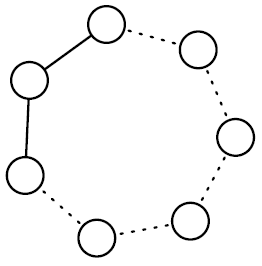
\includegraphics[height=.2\textwidth]{Figuras/graph5.png}
        \end{minipage}
        \caption{}
     \end{subfigure}
     \begin{subfigure}[b]{0.3\textwidth}
        \begin{minipage}{7cm}
       	 \centering% El subgrafo está centrado
	    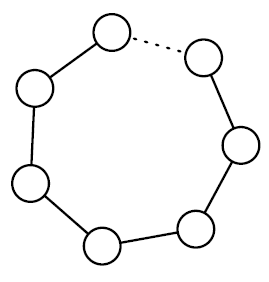
\includegraphics[height=.2\textwidth]{Figuras/graph6.png}
        \end{minipage}
        \caption{}
     \end{subfigure}
     \caption{Ejemplos de gráficas circulares.}
    \label{figura:2.5}
\end{figure}

Podemos descartar a las gráficas que no tienen ninguna arista punteada por que son de tipo $\tilde{A}_{m}$, es decir, no son positivas. Denotemos con $C\left(n\right)$ a el grafo circular de $n$ vértices que tiene exactamente una arista punteada $x_{n} \tikz[baseline=-0.1ex]\draw [dotted] (0,0.05) -- (1,0.05); x_{1}$ y las demás sólidas:

\begin{figure}[h]
   \centering% El subgrafo está centrado
   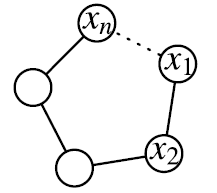
\includegraphics[width=2cm]{Figuras/graph7.png}
\end{figure}

Con el algoritmo \ref{alg:algoritmoInflaciones} podemos comprobar directamente que $C\left(4\right)$ tiene tipo Dynkin $D_{4}$. Si $n \ge 4$, aplicando la inflación $T_{n 1}^{-}$ y borrando el vértice $x_{n}$ de $C\left(n\right)$ se obtiene $C\left(n - 1\right)$, de modo que por inducción y el teorema \ref{teorema:2.5}, todas las gráficas $C\left(n\right)$ con $n \ge 3$ no pueden ser de tipo $\DynA_{n}$. Hemos mostrado el siguiente lema:\\

\begin{lemma}
Las únicas gráficas circulares $G$ tales que $q_{G}$ es de tipo $\DynA_{n}$ son $F_{3,0}$ y $F_{2,1}$.
\label{lema:2.6}
\end{lemma}
 
Una gráfica es $k$-conexa si no existe ningún subconjunto de $k - 1$ vértices tales que su borrado desconecte a la gráfica. Dicho de otro modo, si $\kappa$ denota la cantidad mínima de vértices que es necesario borrar para obtener una gráfica disconexa, entonces $\kappa \geq k$. Por ejemplo, toda gráfica conexa es automáticamente $1$-conexa y toda gráfica completa $K_{n}$ es $k$-conexa para todo $k \in \{1, 2, \dots, n\}$. De hecho, por definición tenemos que si $G$ es una gráfica $k$-conexa entonces también es $\left(k - 1\right)$-conexa, $\left(k - 2\right)$-conexa, etc. Otro ejemplo: las gráficas circulares son gráficas biconexa($2$-conexos). Ahora supongamos que $\textbf{B}_{q}$ es biconexa y que $q$ es de tipo $\DynA_{n}$; mostraremos que $\textbf{B}_{q}$ es un $\DynA$-bloque.\\

Primero mostraremos que $\textbf{B}_{q}$ debe ser una gráfica completa. Supongamos que no es así y sea $S$ el conjunto de vértices más pequeño tal que al borrarlos de $\textbf{B}_{q}$ la gráfica se vuelve disconexa y defínase $\kappa = |S|$. Sabemos que $\textbf{B}_{q}$ es $2$-conexa, y además que la ausencia de la arista $u \tikz[baseline=-0.1ex]\draw (0,0.05) -- (1,0.05); v$ porque $\textbf{B}_{q}$ no es completa) nos permite obtener una gráfica disconexa borrando todos los vértices excepto $u$ y $v$; por lo tanto tenemos que $2 \leq \kappa \leq n-2$. Seleccionamos cualesquiera $\kappa - 2$ vértices del conjunto $S$ y los borramos de la gráfica $\textbf{B}_{q}$ para obtener otra gráfica $\textbf{B}_{q}^{'}$. Por la definición de $S$ sabemos que $\textbf{B}_{q}^{'}$ es una gráfica biconexa pero no triconexa($3$-conexa). Es decir, en $\textbf{B}_{q}^{'}$ existen dos vértices $x$ e $y$ tales que al borrarlos de $B_{q}^{'}$ se obtiene una gráfica de dos componentes conexos $\mathcal{B}_{0}$ y $\mathcal{B}_{1}$. Consideremos el camino más corto $x \leadsto y$ que inicia en $x$ pasa solamente por vértices de $\mathcal{B}_{0}$ y termina en $y$, juntemos este camino con el camino más corto $y \leadsto x$ que inicia en $y$, pasa solamente por vértices de $\mathcal{B}_{1}$ y termina en $x$. Esta unión forma un ciclo $x \leadsto y \leadsto x$, pero habíamos supuesto que $q$ es de tipo $\DynA_{n}$, por tanto el lema \ref{lema:2.6} nos dice que $\textbf{B}_{q}^{'}$ contiene la siguiente subgráfica inducida (sin tomar en cuenta si las aristas son sólidas o punteadas):\\

\begin{figure}[h]
   \centering% El subgrafo está centrado
   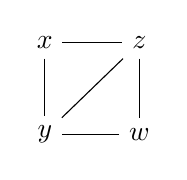
\begin{tikzpicture}
   \node (v0) at (1.37, 0.63) {$x$};
   \node (v1) at (1.37, -0.53) {$y$};
   \node (v2) at (2.57, 0.63) {$z$};
   \node (v3) at (2.57, -0.53) {$w$};
   \draw (v0) -- (v1);
   \draw (v1) -- (v2);
   \draw (v2) -- (v3);
   \draw (v0) -- (v2);
   \draw (v3) -- (v1);
   \end{tikzpicture}
\end{figure}

Aquí $z \in \mathcal{B}_{0}$, $w \in \mathcal{B}_{1}$ y no existe la arista $z \tikz[baseline=-0.1ex]\draw (0,0.05) -- (1,0.05); w$(en otro caso $\textbf{B}_{q}$ seguiría conectada después de quitar los vértices $x$ e $y$). Otra vez mediante el uso del algoritmo \ref{alg:algoritmoInflaciones} se puede demostrar que no importa cuáles aristas sean sólidas o punteadas, esta gráfica no es de tipo $\DynA_{n}$, en contradicción con el teorema \ref{teorema:2.5}; por lo tanto tenemos:\\

\begin{lemma}
Si $q:\mathbb{Z}^{n} \rightarrow \mathbb{Z}$ es una forma unitaria de tipo $\DynA_{n}$ y si $\textbf{B}_{1}$ es una gráfica biconexa, entonces $\textbf{B}_{q}$ es una gráfica completa.
\label{lema:2.7}
\end{lemma}

El siguiente lema se puede leer \textit{entre líneas} en el artículo mencionado; aquí solamente se está recalcando su importancia porque haremos referencia a este lema en capítulos posteriores:

\begin{lemma}
Si toda subgráfica de $\textbf{B}_{q}$ inducida por tres vértices es $F_{3,0}$ o $F_{2,1}$, entonces $\textbf{B}_{q}$ es un $\DynA$-bloque.
\label{lema:2.8}
\end{lemma}

\begin{proof}
Fijemos un vértice $u$ y definamos los conjuntos
\begin{equation*}
\begin{split}
V_{0} & = \{u\} \cup \{v |  \mbox{  existe una arista punteada } u \tikz[baseline=-0.1ex]\draw[dotted] (0,0.05) -- (1,0.05); v\}\\
V_{1} & = \{v |  \mbox{ existe una arista solida } u \tikz[baseline=-0.1ex]\draw (0,0.05) -- (1,0.05); v\}
\end{split}
\end{equation*}
Considérese a otros dos diferentes vértices $v$ y $w$ en $\textbf{B}_{q}$. Por hipótesis tenemos que los vértices $u$, $v$ y $w$ inducen una subgráfica $F_{3,0}$ o $F_{2,1}$. Por la definición de $V_{0}$ y $V_{1}$ concluimos que si dos vértices $v, w$ están en el mismo $V_{i}$ entonces hay una arista punteada $v \tikz[baseline=-0.1ex]\draw[dotted](0,0.05) -- (1,0.05); w$; y en otro caso (están en conjuntos diferentes) hay una arista sólida $v \tikz[baseline=-0.1ex]\draw(0,0.05) -- (1,0.05); w$; por lo tanto $Bq$ es un $\DynA$-bloque.
\end{proof}

Vamos a recapitular lo que hemos visto hasta ahora:\\
\begin{enumerate}
\item El lema \ref{lema:2.7} nos dice que si $q$ es de tipo $\DynA_{n}$ y si $\textbf{B}_{q}$ es biconexa, entonces $\textbf{B}_{q}$ es, de hecho, completa.
\item Pero por el teorema \ref{teorema:2.5} cada subgráfica inducida de $B_{q}$ debe definir otra forma de tipo $\DynA_{n}$.
\item En particular, como $\textbf{B}_{q}$ es completa, el lema \ref{lema:2.6} nos dice que toda subgráfica inducida por cada tres vértices de $B_{q}$ es $F_{3,0}$ o $F_{2,1}$.
\item Entonces, por lema \ref{lema:2.8} concluimos que $\textbf{B}_{q}$ es un $\DynA$-bloque.
\end{enumerate}

Ahora vamos a mostrar el recíproco: que todo $\DynA$-bloque es biconexo y que define una forma de tipo $\DynA_{n}$. La biconexidad es obvia puesto que todo $\DynA$-bloque $F_{m, m}$ es una gráfica completa. Ahora bien, renombremos a los vértices en $V_{0}$ como $x_{1}, x_{2}, \ldots, x_{m}$; y a los de $V_{1}$ como $x_{m+1}, x_{m+2}, \ldots, x_{n}$. Podemos “deshilar” a $\textbf{B}_{q}$ en dos etapas: en la primera quitamos todas las aristas punteadas que hay entre los vértices de $V_{1}$ usando las inflaciones $T_{i i+1}^{-}$ en orden $i = n-1, n-2, \ldots, m+1$ y en la segunda las punteadas que hay en $V_{0}$ usando las inflaciones $T_{i+1 i}^{-}$ en orden $i = 1, 2, \dots, m-1$.\\

Para mostrar que este método de “deshilado” funciona, supongamos que $m \ge 0$ y $m^{'} \ge 0$ y sean $V_{0} = \{x_{1}, \ldots, x_{m}\}$ y $V_{1} = \{x_{m+1}, \ldots, x_{n}\}$ los conjuntos que definen a $F_{m,m^{'}}$ . Sea $x_{r}$ incidente en $x_{n-1}$.

\begin{itemize}
\item Si $x_{r} = x_{n}$ entonces la arista $x_{n-1} \tikz[baseline=-0.1ex]\draw [dotted] (0,0.05) -- (1,0.05); x_{n}$ se sustituye por $x_{n-1} \tikz[baseline=-0.1ex]\draw (0,0.05) -- (1,0.05); x_{n}$.
\item Para todos los $x_{r}$ tales que exista una arista punteada $x_{r} \tikz[baseline=-0.1ex]\draw [dotted] (0,0.05) -- (1,0.05); x_{n-1}$ se tiene que $x_{r} \in V_{1}$ y el arrastre forma una arista sólida $x_{r} \tikz[baseline=-0.1ex]\draw (0,0.05) -- (1,0.05); x_{n}$ que se cancela con la arista $x_{r} \tikz[baseline=-0.1ex]\draw [dotted] (0,0.05) -- (1,0.05); x_{n}$; por lo tanto luego de aplicar $T_{n-1 n}^{-}$ en el vértice $x_{n}$ no incide ninguna arista punteada.
\item Para todos los $x_{r}$ tales que exista una arista sólida $x_{r} \tikz[baseline=-0.1ex]\draw (0,0.05) -- (1,0.05); x_{n-1}$ se tiene que $x_{r} \in V_{0}$ y el arrastre forma una arista punteada $x_{r} \tikz[baseline=-0.1ex]\draw [dotted] (0,0.05) -- (1,0.05); x_{n}$ que se cancela con la arista $x_{r} \tikz[baseline=-0.1ex]\draw (0,0.05) -- (1,0.05); x_{n}$; por lo tanto luego de aplicar $T_{n-1 n}^{-}$ en el vértice $x_{n}$ no incide ninguna arista sólida.
\end{itemize}

De lo anterior concluimos que al aplicar $T_{n-1 n}^{-}$ a $F_{m, m^{'}}$ se obtiene $F_{m, m^{'}-1}$ unida con una arista sólida $x_{n-1} \tikz[baseline=-0.1ex]\draw (0,0.05) -- (1,0.05); x_{n}$; luego entonces por inducción se sigue la sucesión de inflaciones $\left(T_{i i+1}^{-}\right)_{i=n-1}^{m+1}$ sobre el grafo $F_{m,m^{'}}$ produce la gráfica $F_{m,1}$ unido con $x_{m+1} \tikz[baseline=-0.1ex]\draw (0,0.05) -- (1,0.05); \cdots \tikz[baseline=-0.1ex]\draw (0,0.05) -- (1,0.05);  x_{n}$. Un razonamiento similar muestra que la sucesión de inflaciones $\left(T_{i+1 i}^{-}\right)_{i=1}^{m-1}$ aplicadas a $F_{m,1}$ produce $F_{m,m^{'}}$. Por lo tanto el método descrito transforma $F_{m,m^{'}}$ en $\DynA_{m,m^{'}}$. *

\begin{figure}[h]
    \begin{subfigure}[b]{0.3\textwidth}
      \begin{minipage}{7cm}
	\centering% El subgrafo está centrado
	    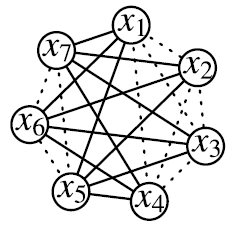
\includegraphics[height=.2\textwidth]{Figuras/graph8.png}
	 \end{minipage}
	\caption{Original}
     \end{subfigure}
     \begin{subfigure}[b]{0.3\textwidth}
        \begin{minipage}{7cm}
       	 \centering% El subgrafo está centrado
	    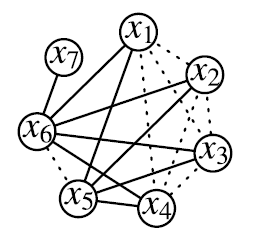
\includegraphics[height=.2\textwidth]{Figuras/graph9.png}
        \end{minipage}
        \caption{$T_{6 7}^{-}$}
     \end{subfigure}
     \begin{subfigure}[b]{0.3\textwidth}
        \begin{minipage}{7cm}
       	 \centering% El subgrafo está centrado
	    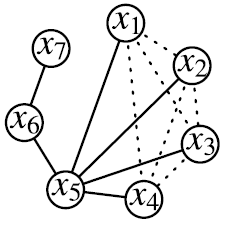
\includegraphics[height=.2\textwidth]{Figuras/graph10.png}
        \end{minipage}
        \caption{$T_{5 6}^{-}$}
     \end{subfigure}
      \begin{subfigure}[b]{0.3\textwidth}
      \begin{minipage}{7cm}
	\centering% El subgrafo está centrado
	    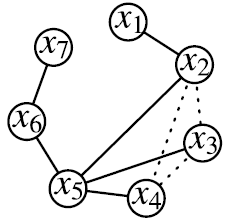
\includegraphics[height=.2\textwidth]{Figuras/graph11.png}
	 \end{minipage}
	\caption{$T_{2 1}^{-}$}
     \end{subfigure}
     \begin{subfigure}[b]{0.3\textwidth}
        \begin{minipage}{7cm}
       	 \centering% El subgrafo está centrado
	    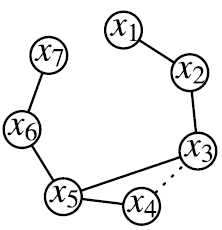
\includegraphics[height=.2\textwidth]{Figuras/graph12.png}
        \end{minipage}
        \caption{$T_{3 2}^{-}$}
     \end{subfigure}
     \begin{subfigure}[b]{0.3\textwidth}
        \begin{minipage}{7cm}
       	 \centering% El subgrafo está centrado
	    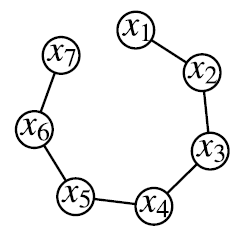
\includegraphics[height=.2\textwidth]{Figuras/graph13.png}
        \end{minipage}
        \caption{$T_{4 3}^{-}$}
     \end{subfigure}
     \caption{Deshilando $F_{4, 3}$}
    \label{figura:2.6}
\end{figure}

Se ha demostrado lo siguiente:
\begin{lemma}
$q$ es una forma unitaria de tipo $\DynA_{n}$ con $\textbf{B}_{q}$ biconexa si y solamente si $\textbf{B}_{q}$ es un $\DynA$-bloque.
\label{lemma:2.9}
\end{lemma}

\textbf{ENSAMBLAJE DE FORMAS $\DynA_{n}$}

Ahora sí tenemos las herramientas necesarias para justificar el ensamble de $\DynA$-bloques. Primero veamos que todo ensamble de $\DynA$-bloques en verdad define una forma unitaria de tipo $\DynA_{n}$.\\

Supongamos que $T$ es el árbol que subyace en un pegado de $\DynA$-bloques. Si este árbol tiene un solo vértice entonces ya acabamos por el lema 2.9 recién mostrado. En otro caso, como $T$ es un árbol, debe haber un vértice $t$ de grado $1$ (podría decirse que t es una hoja del árbol). Entonces el $\DynA$-bloque asociado al vértice $t$, que es $\mathcal{B}_{t} = F_{m, m^{'}}$ , comparte exactamente un vértice $v$ con algún otro $\DynA$-bloque  $\mathcal{B}_{s}$(*). Ahora apliquemos la técnica deshilado explicada justo antes del lema \ref{lemma:2.9}, pero renombrando al vértice $v$ como $x_{m, m^{'}}$ , de manera que este deshilado no afecta en absoluto a ningún otro vértice de $\mathcal{B}_{s}$. Lo que veremos (*) es que ahora del vértice $v$ “cuelga” la siguiente gráfica:

\begin{figure}[h]
    \begin{subfigure}[b]{0.2\textwidth}
      \begin{minipage}{4cm}
	\centering% El subgrafo está centrado
	    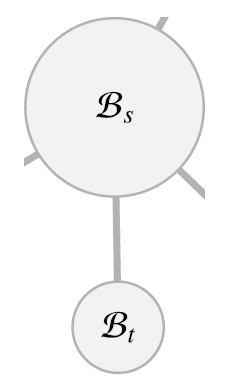
\includegraphics[height=.4\textwidth]{Figuras/graph20.png}
	 \end{minipage}
	 \caption{}
     \end{subfigure}
     \begin{subfigure}[b]{0.2\textwidth}
        \begin{minipage}{4cm}
       	 \centering% El subgrafo está centrado
	    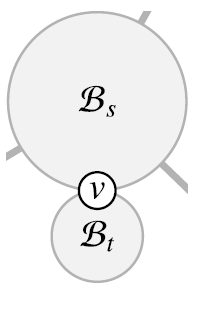
\includegraphics[height=.4\textwidth]{Figuras/graph21.png}
        \end{minipage}
        \caption{}
     \end{subfigure}
     \begin{subfigure}[b]{0.2\textwidth}
        \begin{minipage}{4cm}
       	 \centering% El subgrafo está centrado
	    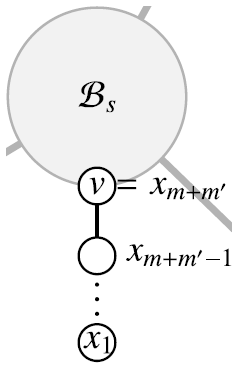
\includegraphics[height=.4\textwidth]{Figuras/graph22.png}
        \end{minipage}
        \caption{}
     \end{subfigure}
      \begin{subfigure}[b]{0.2\textwidth}
      \begin{minipage}{4cm}
	\centering% El subgrafo está centrado
	    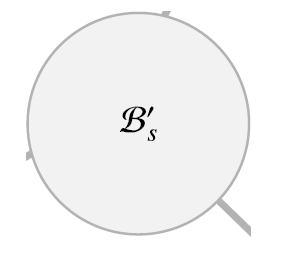
\includegraphics[height=.4\textwidth]{Figuras/graph23.png}
	 \end{minipage}
	 \caption{}
     \end{subfigure}
     \caption{Esquemática de la fusión de dos $\DynA$-bloques}
    \label{figura:2.7}
\end{figure}

\begin{equation*}
x_{m+m^{'}} \tikz[baseline=-0.1ex]\draw (0,0.05) -- (1,0.05); x_{m+m^{'}-1} \tikz[baseline=-0.1ex]\draw (0,0.05) -- (1,0.05); \cdots \tikz[baseline=-0.1ex]\draw (0,0.05) -- (1,0.05); x_{3} \tikz[baseline=-0.1ex]\draw (0,0.05) -- (1,0.05); x_{2} \tikz[baseline=-0.1ex]\draw (0,0.05) -- (1,0.05); x_{1}
\end{equation*}

Esto se parece a lo que se obtiene durante los pasos intermedios para deshilar un $\DynA$-bloque; esto sugiere hacer el proceso inverso, es decir, utilizar las deflaciones.\\

Podemos usar las deflaciones para “tejer” los vértices de $\mathcal{B}_{t}$ en $\mathcal{B}_{s}$ aplicando sucesivamente $T_{i+1, i}$ en orden $i = m + m^{'} - 1, m + m^{'} - 2, \ldots, 3, 2, 1$ (porque precisamente este es el proceso inverso al de deshilado). Cada vez que hacemos esto estamos, en cierto sentido, agregando $x_{i}$ a $\mathcal{B}_{s}$; de manera que al término de estas deflaciones tendremos todos los vértices de $\mathcal{B}_{s}$ y $\mathcal{B}_{t}$ en un mismo $\DynA$-bloque $\mathcal{B}_{s}^{'}$. Así hemos mostrado cómo fusionar dos $\DynA$-bloques del árbol en uno solo, repitiendo este proceso podemos fusionarlos todos, mostrando así que todo ensamble de $\DynA$-bloques es equivalente a un solo $\DynA$-bloque. *

\begin{figure}[h]
    \begin{subfigure}[b]{0.2\textwidth}
      \begin{minipage}{4cm}
	\centering% El subgrafo está centrado
	    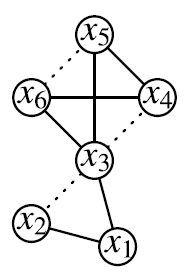
\includegraphics[height=.4\textwidth]{Figuras/graph14.png}
	 \end{minipage}
	\caption{Original}
     \end{subfigure}
     \begin{subfigure}[b]{0.2\textwidth}
        \begin{minipage}{4cm}
       	 \centering% El subgrafo está centrado
	    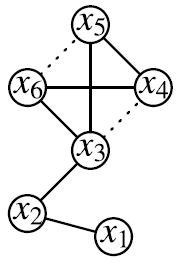
\includegraphics[height=.4\textwidth]{Figuras/graph15.png}
        \end{minipage}
        \caption{$T_{2 3}^{-}$}
     \end{subfigure}
     \begin{subfigure}[b]{0.2\textwidth}
        \begin{minipage}{4cm}
       	 \centering% El subgrafo está centrado
	    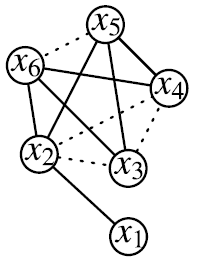
\includegraphics[height=.4\textwidth]{Figuras/graph16.png}
        \end{minipage}
        \caption{$T_{3 2}^{+}$}
     \end{subfigure}
      \begin{subfigure}[b]{0.2\textwidth}
      \begin{minipage}{4cm}
	\centering% El subgrafo está centrado
	    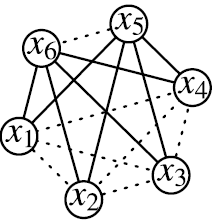
\includegraphics[height=.4\textwidth]{Figuras/graph17.png}
	 \end{minipage}
	\caption{$T_{2 1}^{+}$}
     \end{subfigure}
     \caption{Ejemplo de fusión de dos $\DynA$-bloques}
    \label{figura:2.8}
\end{figure}

\begin{lemma}
Si $G$ es una gráfica construida por un ensamble de árbol de $\DynA$-bloques, entonces $q_{G}$ es de tipo $\DynA_{n}$.
\label{lemma:2.10}
\end{lemma}

Falta mostrar el converso: que si $G$ es una forma unitaria con tipo Dynkin $\DynA_{n}$ entonces se puede construir mediante un ensamble de árbol de $\DynA$-bloques. Una \textbf{componente biconexa} de una gráfica, es una subgrafo biconexo maximal (no contenida propiamente en ninguna otra subgrafo biconexo). La manera más fácil de entender a las componentes biconexos es mediante los \textbf{puntos de articulación}, que son los vértices de la gráfica que al quitarlos la deja desconectada.\\

\begin{figure}[h]
    \begin{subfigure}[b]{0.5\textwidth}
      \begin{minipage}{7cm}
	\centering% El subgrafo está centrado
	    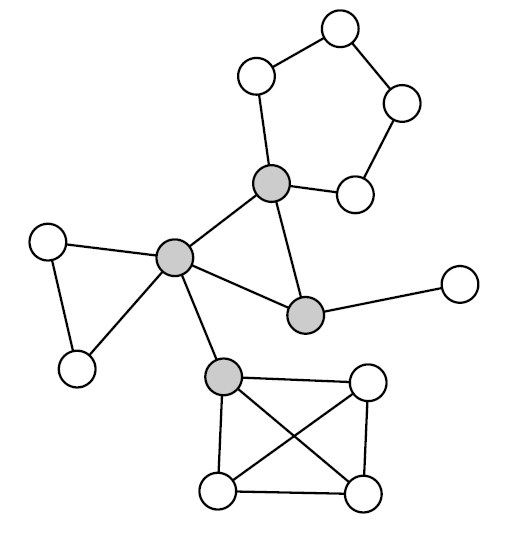
\includegraphics[height=.5\textwidth]{Figuras/graph18.png}
	 \end{minipage}
	\caption{}
     \end{subfigure}
     \begin{subfigure}[b]{0.5\textwidth}
        \begin{minipage}{7cm}
       	 \centering% El subgrafo está centrado
	    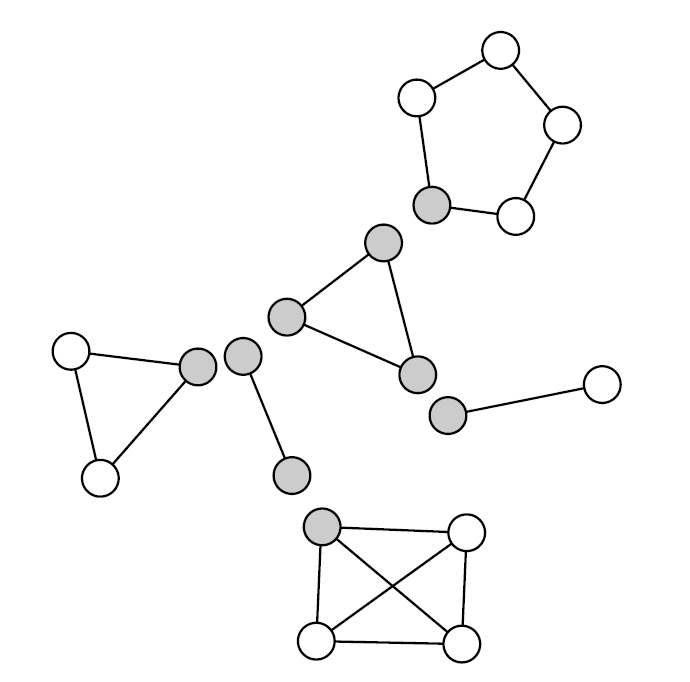
\includegraphics[height=.5\textwidth]{Figuras/graph19.png}
        \end{minipage}
        \caption{}
     \end{subfigure}
     \caption{Una gráfica sus puntos de articulación y componentes biconexas}
    \label{figura:2.9}
\end{figure}

\begin{lemma}
Las componentes biconexas de una gráfica particionan al conjunto de aristas.
\label{lemma:2.11}
\end{lemma}

\begin{proof}
Cada arista es por sí misma una subgrafica biconexa, y por lo tanto pertenece a una subgrafica biconexa maximal; por otro lado ninguna arista puede pertenecer a dos componentes biconexas, por que si este fuera el caso entonces podríamos pegar ambas componentes por medio de la arista que tienen en común, mostrando así que no eran maximales.
\end{proof}

Del teorema \ref{teorema:2.5} y del lema \ref{lemma:2.9} se concluye que si $q$ es de tipo $\DynA_{n}$ entonces las componentes biconexas de $\textbf{B}_{q}$ son $\DynA$-bloques. Supongamos que $\mathcal{B}_{1}, mathcal{B}_{2}, \ldots, \mathcal{B}_{t}$ son las componentes biconexas de $\textbf{B}_{q}$, y formemos una nueva gráfica $T$ de vértices $\{1, 2, \ldots, t\}$, donde cada arista $i \tikz[baseline=-0.1ex]\draw (0,0.05) -- (1,0.05); j$ representa que $\mathcal{B}_{i}$ y $\mathcal{B}_{j}$, con $i \neq j$, tienen un vértice en común (este debe ser un punto de articulación de $\textbf{B}_{q}$). Más aún, si $\mathcal{B}_{i}$ y $\mathcal{B}_{j}$ comparten el vértice $v$ definiremos $\sigma_{i}\left(i \tikz[baseline=-0.1ex]\draw (0,0.05) -- (1,0.05); j\right) = \sigma_{j}\left(i \tikz[baseline=-0.1ex]\draw (0,0.05) -- (1,0.05); j\right) = v$.\\

Debido a la manera en que construimos las funciones $\sigma_{k}$ y la gráfica $T$, tenemos que las siguientes tres afirmaciones son equivalentes:\\

\begin{enumerate}
\item Cada función $\sigma_{k}$ es inyectiva
\item $T$ es un árbol
\item Ningún punto de articulación pertenece a tres o más componentes biconexas
\end{enumerate}

Por lo tanto basta mostrar cualquiera de estas afirmaciones. Mostraremos la tercera afirmación por inducción. Si $\textbf{B}_{q}$ no tiene puntos de articulación, por vacuidad ningún punto de articulación pertenece a tres o más componentes biconexas. Ahora supongamos que $\textbf{B}_{q}$ tiene al menos un punto de articulación $v$; entonces $\textbf{B}_{q} - v$ tiene componentes conexas $\mathcal{C}_{1}, \mathcal{C}_{2}, \ldots, \mathcal{C}_{\ell}$. Defínase $D_{i}$ como la subgráfica de $\textbf{B}_{q}$ inducida por los vértices $V\left(\mathcal{C}_{i}\right) \cup \{v\}$. Por teorema \ref{teorema:2.5} cada $q_{\mathcal{C}_{i}}$ es de tipo $\DynA_{n_{i}}$ y por hipótesis de inducción, cada $C_{i}$ se construye haciendo un ensamble de árbol de $\DynA$-bloques (ningún $\mathcal{C}_{i}$ tiene puntos de articulación que pertenezcan a tres o más componentes biconexas). Ahora, mediante el proceso previamente descrito, deshilemos a cada $\mathcal{C}_{i}$ para convertirlo en un grafo $\DynA_{n_{i}}$ que tenga a $v$ como extremo. Luego entonces $v$ es el centro de una gráfica de estrella de $\ell$ picos y sin aristas punteadas; pero habíamos supuesto que $\textbf{B}_{q}$ es de tipo $\DynA$, de manera que el algoritmo \ref{alg:algoritmoInflaciones} nos dice que $\ell = 2$. Por lo tanto $v$, que es un punto de articulación cualquiera, solamente puede pertenecer a exactamente dos componentes biconexas.\\

Así tenemos el siguente teorema:\\

\begin{theorem}
Una forma unitaria $q$ es de tipo $\DynA_{n}$ si y solamente si $\textbf{B}_{q}$ se construye mediante un ensamble de árbol de $\DynA$-bloques.
\label{teorema:2.12}
\end{theorem}

Sin embargo, para los fines de este trabajo es más conveniente reinterpretar este resultado utilizando otras palabras (pero la demostración es la misma):

\begin{corollary}
Una forma unitaria $q$ es de tipo $\DynA_{n}$ si y solo si $\textbf{B}_{q}$ es conexa, sus componentes biconexas son $\DynA$-bloques y todo punto de articulación pertenece a exactamente dos de estas componentes.
\label{corolario:2.13}
\end{corollary}
